\documentclass[sigconf]{acmart}

% A4 instead of letter paper
\geometry{a4paper}

\usepackage[ngerman]{babel}
\usepackage{times}

\usepackage{booktabs} % More formal table style.

\usepackage[T1]{fontenc}
\usepackage[utf8]{inputenc}
\usepackage{caption}
\captionsetup[table]{position=bottom} 


% ACM style ``tweaking''
\settopmatter{printacmref=false}                   % Removes citation information below abstract; but causes a warning when compiling a document with more than one page
\renewcommand\footnotetextcopyrightpermission[1]{} % Removes footnote with conference information in first column
\pagestyle{plain}                                  % Removes running headers

% Figures
\DeclareGraphicsRule{.ai}{pdf}{*}{}% Handle .ai files as .pdf files.
\DeclareGraphicsExtensions{.pdf,.ai,.jpg,.png}
\pdfpagebox 5% Use ArtBox instead MediaBox. 1=MediaBox, 2=CropBox, 3=BleedBox, 4=TrimBox, 5=ArtBox. (shell: pdfinfo -box <pdf-file>)
\setkeys{Gin}{pagebox=artbox}% Alternative (necessary for newer tex versions) for \pdfpagebox 5 in preceding line.
\graphicspath{{../report-template-figures/}}

\acmConference{Algorithm Engineering}{Winter term 2024/25}{Jena, Germany}

\usepackage{fancyhdr}  
\pagestyle{fancy}  
\fancyhf{}  
\fancyfoot[C]{\thepage} % Seitenzahl zentriert in der Fußzeile
\renewcommand{\headrulewidth}{0pt}  
\renewcommand{\footrulewidth}{0pt}  
\settopmatter{printfolios=true}
\setlength{\footskip}{40pt}

\begin{document}
\pagenumbering{arabic}
\thispagestyle{fancy}
\settopmatter{printfolios=true}

\title{Raytracer}
\subtitle{Algorithm Engineering}         % Optional.

\author{Nele Rissiek}
\author{Robert Scheer}
\affiliation{%
    \institution{Friedrich-Schiller-Universität Jena}
    \city{Jena}
    \country{Germany}
}
\email{nele.rissiek@uni-jena.de}
\email{robert.scheer@uni-jena.de}

\begin{abstract}
In diesem Paper wird die Entwicklung eines Raytracers beschrieben, der auf datenorientierter Programmierung basiert.
Der Fokus liegt auf der Optimierung der Performance durch die Umstellung von einer objektorientierten auf eine datenorientierte Architektur.
Zusätzlich wird die Implementierung von SIMD-Vektorisierung zur Parallelisierung von Berechnungen behandelt.
Auch wird die Performance des Raytracers anhand von Skalierungstests analysiert.
Insbesondere wird bei der Untersuchung auf den Einfluss verschiedener Parameter wie Auflösung, Supersampling, Bounces und Scatter eingegangen und wie diese Parameter die Laufzeit und Bildqualität beeinflussen.
Die Ergebnisse zeigen, dass vor allem die Auflösung und die Anzahl an Supersampling-Schritten maßgeblichen Einfluss auf die Laufzeit haben. Die Scatter und Bounces haben vorallem bei komplexeren Scenen eine grosse Auswirkung.
Die gewonnenen Erkenntnisse bieten eine Grundlage für die Optimierung von Raytracing-Algorithmen in Hinblick auf Performance und Bildqualität.
 \end{abstract}

\maketitle
\section{Einleitung} \label{Einleitung}
Raytracing ist ein grundlegendes Verfahren zur realistischen Bildsynthese, das insbesondere in der Computergrafik und Filmindustrie Anwendung findet.
Die Technik simuliert die Ausbreitung von Lichtstrahlen in einer Szene, um Schatten, Reflexionen und Lichtbrechungen physikalisch korrekt darzustellen.

Die Herausforderung besteht darin, die Performance des Algorithmus zu optimieren, ohne die Bildqualität zu beeinträchtigen.
In diesem Paper wird ein Raytracer vorgestellt, der gezielt durch datenorientierte Programmierung und SIMD-Vektorisierung sowie OpenMP-Parallelisierung optimiert wurde.
Ziel der Arbeit ist es, die Laufzeit des Renderprozesses zu minimieren, indem die Vorteile moderner Prozessorarchitekturen ausgenutzt werden.
Außerdem wird der Einfluss verschiedener Parameter auf die Laufzeit und Bildqualität untersucht, um ein besseres Verständnis für die Skalierbarkeit und Optimierungsmöglichkeiten des Raytracing-Verfahren zu gewinnen.

Zunächst wird die grundlegende Architektur des Raytracers beschrieben.
Anschließend erfolgt eine detaillierte Betrachtung der Umstellung von objektorientierter auf datenorientierte Programmierung.
Danach wird die Integration von SIMD-Vektorisierung erläutert.
Abschließend werden die Ergebnisse der Performanceoptimierung präsentiert und diskutiert.

\section{Der Algorithmus} \label{Algorithmus}  % Change title accordingly
\subsection{3D-Szenenbeschreibung} \label{Szenenbeschreibung}
Zur Definition der 3D-Szene wurde ein eigens entwickelter XML-Parser implementiert.
Die Wahl von XML als Beschreibungssprache erfolgte aufgrund der guten Lesbarkeit für Menschen, der maschinellen Verarbeitbarkeit sowie der hohen Flexibilität bei der Darstellung hierarchischer Strukturen.
Zusätzlich wurden auch die Rendereinstellungen in XML hinterlegt, um ein einheitliches, sowohl menschen- als auch maschinenlesbares Format zu gewährleisten.
Dies erleichtert die Konfiguration und ermöglicht eine klare Trennung zwischen Szenenbeschreibung und Renderlogik.

\subsection{Objektorientierte Struktur} \label{OOP}
Nach dem Einlesen der XML-Daten erfolgt die Abbildung der 3D-Szene in einer objektorientierten (OOP) Datenstruktur.
Diese Entscheidung für eine OOP-Datenstruktur wurde getroffen, da sie eine intuitive Abbildung der Szeneobjekte sowie eine einfache Änderbarkeit von Attributen ermöglicht.
Objekte wie Kugeln, Ebenen oder die Kamera werden hierbei als eigenständige Klassen modelliert, wobei die Eigenschaften und Methoden der Objekte gekapselt werden.


Es zeigte sich jedoch, dass eine OOP-Struktur starke Nachteile beim Rendern hat.
Insbesondere bei den milliardenzahlreichen Funktionsaufrufen während der Raytracing-Berechnungen stellt der wiederholte Zugriff auf Objektattribute über Getter-Methoden eine erhebliche Laufzeitbelastung dar. 
Deswegen werden die gesamten Daten vor dem Rendern in eine datenorientierte Struktur konvertiert.
Die Evaluation (siehe Abschnitt \ref{Evaluation}) liefert eine detaillierte Analyse der Performanceunterschiede zwischen einer OOP-Struktur und einer DO-Struktur beim Rendern.

Vor der eigentlichen Renderingphase werden die Vektoren zur Darstellung von Positionen und Richtungen in \_{m128} SIMD-Registrierungen (Single Instruction Multiple Data) umgewandelt.
Hierbei entfällt auch die OOP-Struktur zugunsten einer optimierten, datenorientierten Speicherung.

\subsection{Kernelfunktion} \label{Kernelfunktion}
Das Verhalten jedes Pixels wird durch eine zentrale Kernelfunktion definiert.
Diese Funktion ermöglicht es, unterschiedliche Renderverfahren schnell und modular zu testen, wodurch das Debuggen von neuen Features problemlos funktioniert.
Beispielhafte Implementierungen der Kernelfunktion umfassen vollständiges Raytracing, Raytracing ohne Reflexionen oder die reine Entfernungsmessung zwischen Kamera und Szenenobjekten.
Während des Renderprozesses wird für jeden Pixel die Kernelfunktion aufgerufen, sodass eine Steuerung des Renderverhaltens gewährleistet ist.

Die einzelnen Pixel-Zeilen des Bildes werden durch OpenMP parallelisiert.

\subsection{Finaler Raytracing-Kernel} \label{finalerKernel}
Der finale Raytracing-Kernel implementiert ein Supersampling-Verfahren zur Reduktion von Aliasing-Effekten.
Dabei wird für jeden Pixel eine Menge von Strahlen (Rays) an leicht versetzten Positionen innerhalb des Pixels erzeugt.
Die Farbwerte dieser Strahlen werden anschließend gemittelt und danach ein Gauß-Filter angewendet, wodurch eine Kantenglättung erzielt wird.
Je mehr Strahlen pro Pixel verwendet werden, desto weicher und realistischer wird das Bild, allerdings steigt der Rechenaufwand dementsprechend an.

Obwohl es leistungsfähigere Anti-Aliasing- und De-Noising-Algorithmen gibt, wurde Supersampling aufgrund seiner einfachen Implementierbarkeit gewählt.
Die Rekursionstiefe der Strahlen stellt dabei die Anzahl an Reflexionen (Bounces), die ein einzelner Strahl maximal durchführen darf, dar.

Für jeden Lichtstrahl werden sämtliche Szenenobjekte auf Kollisionen geprüft.
Die nächstgelegene Kollision bestimmt den Ursprung der Folgestrahlen.
Die Grundfarbe des getroffenen Objekts wird zur Farbe des aktuellen Rays addiert, wobei materialabhängige Eigenschaften berücksichtigt werden.

\subsection{Erstellung neuer Rays} \label{ErstellungRays}
Die Anzahl der nachfolgenden Rays hängt von der Qualitätseinstellung ab.
Im Kollisionspunkt werden neue Rays erzeugt, deren Richtung durch die Materialeigenschaften des getroffenen Objekts bestimmt wird.
Glänzende Materialien erzeugen spiegelnde Reflexionen entlang der Oberflächennormalen, während matte Materialien diffuse Reflexionen generieren.
Die Lambertian-Reflexion beschreibt die ideale diffuse Reflektion auf einer rauen Oberfläche.
Hierbei wird das einfallende Licht kosinusverteilt in alle Richtungen gestreut.
Das Reflektionsverhalten sagt hier aus, dass das Licht in Richtung der Oberflächennormalen am Stärksten reflektiert wird und zu den Seiten hin schwächer erscheint, also ideal zur Modellierung von matten Materialien.

Zur Simulation physikalisch realistischer Streuprozesse wird jeder neue Ray mit einer Zufallskomponente versehen. Die Generierung der Zufallsvektoren erfolgt mit SIMD-Operationen.
Die Stärke dieser Komponente ist proportional zur Rauheit des Materials: Ein idealer Spiegel besitzt eine geringe Streuung, während raue Oberflächen wie gebürstetes Aluminium eine stärkere zufällige Abweichung aufweisen.

Mit jedem Rekursionsschritt nimmt die Anzahl der neu erzeugten Rays bei einer Kollision ab, da der Einfluss tieferer Rekursionen auf das Endergebnis sehr gering ist.
Diese sinkende Strahlenerzeugung dient der Effizienzsteigerung, da kaum sichtbare Farbänderungen vermieden werden, während der Gesamtaufwand reduziert wird.

\subsection{Ausgabe der Daten} \label{AusgabeDaten}
Die Ausgabe der gerenderten Bilddaten erfolgt im ASCII-PPM-Format (Portable Pixel Map).
Dieses Dateiformat ermöglicht eine einfache, sequentielle Speicherung der Farbwerte jedes Pixels in einer Textdatei.
Die Wahl des ASCII-Formats wurde aufgrund seiner einfachen Implementierung, Menschenlesbarkeit und verlustfreien Datenspeicherung getroffen.
Jeder Pixelwert wird in Klartext als drei Ganzzahlen (Rot-, Grün- und Blauanteil) zwischen 0 und 255 bzw. 0 und 65536 hinterlegt, was eine direkte Inspektion der Bilddaten erlaubt.

\subsection{Laufzeitabschätzungen} \label{Laufzeit}
Die Laufzeit des Raytracers hängt von einigen Faktoren ab:
Die Anzahl der Objekte in der Szene beeinflusst die Laufzeit linear, da jedes Objekt bei der Kollisionsprüfung berücksichtigt werden muss.
Die Auflösung des gerenderten Bildes skaliert ebenfalls linear, da die Anzahl der zu berechnenden Pixel direkt proportional zur Bildgröße ist.
Eine quadratische Erhöhung der Laufzeit wird durch die Verwendung von Supersampling erzeugt, da pro Pixel eine Vielzahl von Rays erzeugt und verarbeitet werden.
Die maximale Anzahl der Reflektionen wirkt sich je nach Anordnung der Szenenobjekte exponentiell auf die Laufzeit aus, da jeder Ray potenziell neue Rekursionen erzeugt.
Zudem führt die Streuungskomponente (Scatter) zu einer weiteren exponentiellen Erhöhung der Laufzeit, da für jeden Ray zusätzliche Strahlen generiert werden.
Die Scatter-Reduktion wirkt im Besten Fall invers exponentiell, da mit zunehmender Rekursionstiefe weniger neue Strahlen erzeugt werden, um die Gesamtrechenzeit zu optimieren.

\subsection{Animation} \label{Animation}
Die Animation der gerenderten Bildsequenzen erfolgt durch ein externes und unabhängiges Python-Programm.
Aufgrund seiner leichten Implementierung und der unkomplizierten Datei-I/O-Operationen wurde Python ausgewählt.
Das Programm simuliert 10 perfekt elastische Kugeln, die in einer Box miteinander kollidieren und in der Gegend herumspringen.
Nachdem die Positionen der Kugeln für einen Zeitschritt berechnet wurden, werden die Positionen in das Szenen-XML Format geschrieben.
Anschließend wird der Raytracer automatisiert gestartet, um die entsprechenden Einzelbilder zu erzeugen.
Nach Abschluss aller Renderingprozesse werden die generierten PPM-Bilder mittels ffmpeg zu einem MP4-Video zusammengeführt.
Dieses Verfahren ermöglicht eine effiziente und einfache Erstellung von Videosequenzen.

\section{Evaluation} \label{Evaluation}
\subsection{Objektorientiert vs. Datenorientiert} \label{OOP_DO}
Vor der Umstellung auf die Datenorientiere Szenenstruktur in der Renderschleife mussten die Szenenobjekte in der Renderschleife gecastet werden. Das war sehr teuer.
Die Laufzeit betrug hierbei in einer vordefinierten Testszene durchschnittlich 23 Sekunden.
Nun bestand die Idee, die benötigten Daten aus der OOP-Struktur direkt in den Speicher zu legen, um unnötige Downcasts und Aufrufe von Getter-Methoden durch direkten Speicherzugriff zu vermeiden. Zudem wird die Cache-Nutzung optimiert, da alle benötigten Daten eng beieinander liegen.
Der benötigte Speicherplatz, der pro Objekt benötigt wird, kann man Tabelle \ref{SpeichergrößeObjekt} entnommen werden.

\begin{table}[b]
 \caption{Speichergröße pro Objekt}

 \label{SpeichergrößeObjekt}
 \centering
 \small
 \begin{tabular}[h]{lcccr}
  \toprule
  Information & Memory Size in Bytes & Memory Adress\\
  \midrule
  Object Type ID & 1 (char) & 0\\
  Object Position & 4 (Vector) * 4 (float) & 4\\
  Object Scale & 4 (Vector) * 4 (float) & 20\\
  Other Object Attributes & 3 * 4 (Vector) * 4 (float) & 36, 52, 68\\
  Material: Color & 4 (Vector) * 4 (float) & 84\\
  Material: Intensitiy & 4 (float) & 100\\
  Material: Diffuse & 4 (float) & 104\\
  \midrule
  SUM & 108\\
  \bottomrule
 \end{tabular}
\end{table}

Tabelle \ref{SpeichergrößeObjekt} beschreibt die Speicheraufteilung für ein Objekt in einem datenorientierten Renderzyklus. 

Object Type ID speichert die Typerkennung, zum Beispiel Kugel oder Ebene, des Objekts, wodurch eine schnelle Identifikation des Objekttyps garantiert wird.
Object Position speichert die Position des Objektes als Vektor mit vier Floats, wobei jeder Float 4 Byte benötigt.
Die Skalierung des Objektes wird ebenfalls als Vektor mit vier Floats im Attribut Object Scale gespeichert.
Weitere Attribute, wie die Rotation oder zusätzliche Parameter, werden in drei Vektoren mit jeweils vier Floats gespeichert.
Die Farbe des Materials wird in einem Vektor mit vier Floats, die Intensität der Farbe als einzelner Float und der diffuse Lichtanteil des Materials ebenfalls als einzelner Float gespeichert.

Durch die feste Struktur der Speicherbelegungen kann der Zugriff auf die Daten ohne Umwege über Objektmethoden erfolgen.
Das ermöglicht eine schnellere Verarbeitung der Daten, da der Prozessor direkt auf den Speicherbereich zugreifen kann.
Die Gesamtspeichergröße pro Objekt beträgt 108 Bytes, diese Speicherung ist daher besonders für SIMD-Architekturen vorteilhaft, da die Daten in zusammenhängenden Speicherblöcken organsiert sind.
Durch die Organisation der Objekte in eine datenorientierte Struktur konnte die Laufzeit letztendlich auf durchschnittlich 11s (siehe Tabelle \ref{DataOriented} optimiert werden.

\begin{table}[t]
    \caption{Performance Data Oriented}
   
    \label{DataOriented}
    \centering
    \small
    \begin{tabular}[h]{lcr}
        \toprule
        Run 1 & Run 2 & Run 3\\
        \midrule
         11,4s & 11,1s & 10,5s\\
         \bottomrule
    \end{tabular}
\end{table}

\subsection{Vektorisierung} \label{Vektorisierung}
Weiter im Optimierungsprozess kommt es nun zur Anwendung von Vektorisierung auf die vorhandene datenorientierte Struktur. Vor der Vektorisierung wurden Vektoren als drei Gleitkommazahlen dargestellt und Operationen wie Skalierung liefen sequenziell für jede Komponente des Vektors.
Die Laufzeit vor der Vektorisierung der Datenstruktur beträgt im Durchschnitt 11s (Tabelle \ref{DataOriented}).

Zunächst nehmen wir eine simple Vektorisierung vor, hier wurde die SIMD Technologie mittels der xmmintrin.h Header-Bibliothek (SSE-Intrinsics) in die Berechnungen der Vec3 Struktur integriert.
Das ermöglicht, dass mehrere Gleitkommazahlen gleichzeitig in einem einzigen Befehl verarbeitet werden können.
Obwohl die Leistung durch diese Veränderung auf durchschnittlich circa 9,5s verbessert wurde (siehe Tabelle \ref{SimpleVectorization}), bleibt die Optimierung durch die vorhandene Vec3 Struktur begrenzt.
Das bedeutet, dass bei jedem Zugriff eine Konvertierung zwischen der benutzerdefinierten Vec3 Struktur und dem \_m128 SIMD-Datentyp durchgeführt werden muss, was unnötigen Overhead verursacht.

Durch das vollständige Entfernen der Vec3 Struktur wurde dann letztendlich die entscheidende Verbesserung erzielt.
Die Vec3 Struktur wurde vollständig durch statische Methoden ersetzt, die ausschließlich mit dem \_m128 SIMD-Datentyp arbeiten. Außerdem wurden für Positionen statt drei Gleitkommazahlen direkt die \_m128 Strukturen in den Szenen-Speicher abgelegt.
Diese Veränderung vermeidet jeglichen vorher getätigten Konvertierungsaufwand und ermöglicht direkte SIMD-Berechnungen.
Wie Tabelle \ref{EliminationVec3Struct} zu entnehmen, sinkt die Laufzeit hier deutlich auf etwa 5,9s im Durchschnitt, was eine Reduzierung der Renderzeit um fast 50\% im Vergleich zu der Pre-Vectorized Performance bedeutet.

Tabelle \ref{DatenstrukturVektorisierung} zeigt die neue Speicheraufteilung nach der vollständigen Vektorisierung.
Auffällig ist hier, dass die Struktur auf 16-Byte-Alignment optimiert wurde, was genau zu den \_m128 SIMD-Datentypen passt.
Auch wenn die Gesamtspeichergröße pro Objekt nun 112 Bytes, anstatt vorher 108 Bytes, beträgt, sorgt die 16-Byte-Ausrichtung für eine optimale Speicherzugriffszeit, weswegen sich der Zugriff so trotzdem effizienter gestaltet.

\begin{table}[t]
    \caption{Performance simple Vektorisierung}
   
    \label{SimpleVectorization}
    \centering
    \small
    \begin{tabular}[h]{lcr}
        \toprule
        Run 1 & Run 2 & Run 3\\
        \midrule
         9,45s & 9,48s & 9,59s\\
         \bottomrule
    \end{tabular}
\end{table}

\begin{table}[b]
    \caption{Entfernung von Vec3-Strukt}
   
    \label{EliminationVec3Struct}
    \centering
    \small
    \begin{tabular}[h]{lcr}
        \toprule
        Run 1 & Run 2 & Run 3\\
        \midrule
         5,91s & 5,58s & 5,94s\\
         \bottomrule
    \end{tabular}
\end{table}

\begin{table}[b]
 \caption{Datenstruktur nach Vektorisierung}

 \label{DatenstrukturVektorisierung}
 \centering
 \small
 \begin{tabular}[h]{lcccr}
  \toprule
  Information & Memory Size in Bytes & Memory Adress\\
  \midrule
  Object Position & 4 (Vector) * 4 (float) & 0\\
  Object Scale & 4 (Vector) * 4 (float) & 16 (4F)\\
  Other Object Attributes & 3 * 4 (Vector) * 4 (float) & 32 (8F), 48 (12F),\\
  & & 64 (16F)\\
  Material: Color & 4 (Vector) * 4 (float) & 80 (20F)\\
  Material: Intensitiy & 4 (float) & 96 (24F)\\
  Material: Diffuse & 4 (float) & 100 (25F)\\
  Object Type ID & 1 (char) & 104 (26F)\\
  \midrule
  SUM & 112 & (28F)\\
  \bottomrule
 \end{tabular}
\end{table}

\subsection{Skalierungstests}
Das Baseline-Modell, das als Referenzpunkt für die Skalierungstests dient, verwendet eine 720p Auflösung, 2 Supersampling Steps, 2 Bounces und 3 Scatter.
Um die Auswirkungen der Parameter besser erkennen zu können, wurde der Gauß-Filter deaktiviert.
Die folgenden Tabellen zeigen, wie sich einzelne Parameteränderungen auf die Laufzeit des Raytracers auswirken.

In Tabelle \ref{SupersamplingBaseline} wird der Einfluss der Supersampling-Schritte auf die Laufzeit bei einer konstanten Auflösung von 720p untersucht, die anderen Parameter entsprechen denen im Baseline-Modell.
Für jede Konfiguration wurden drei Messungen durchgeführt, um die Stabilität und Konsistenz der Laufzeit zu bewerten.

Die Daten verdeutlichen, dass die Laufzeit mit zunehmender Anzahl an Supersampling-Schritten nahezu exponentiell ansteigt.
Während bei einem Supersampling-Schritt die durchschnittliche Laufzeit bei etwa 3,31 Sekunden liegt, erhöht sich diese bei fünf Schritten auf etwa 20,23 Sekunden.
Dies liegt daran, dass mit jedem zusätzlichen Schritt die Anzahl der pro Pixel ausgesendeten Strahlen steigt, was den Rechenaufwand entsprechend vervielfacht.
\begin{table}[b]
 \caption{Supersampling am Baselinemodell}

 \label{SupersamplingBaseline}
 \centering
 \small
 \begin{tabular}[h]{lcccr}
  \toprule
  Resolution & Supersampling Steps & Run1 & Run2 & Run3\\
  \midrule
  720p & 1 & 3.30s & 3.33s & 3.29s\\
  720p & 2 & 3.66s & 3.64s & 3.71s\\
  720p & 3 & 7.45s & 7.48s & 7.85s\\
  720p & 4 & 12.76s & 13.55s & 13.80s\\
  720p & 5 & 20.14s & 20.11s & 20.43s\\
  \bottomrule
 \end{tabular}
\end{table}
Abbildung \ref{Supersampling1} zeigt das gerenderte Bild mit nur einem Supersampling-Schritt, während Abbildung
\ref{Supersampling5} das Ergebnis mit fünf Supersampling-Schritten darstellt.
Es ist deutlich zu erkennen, dass die Bildqualität bei mehr Supersampling-Schritten erheblich verbessert wird, insbesondere in Form von weniger sichtbarem Rauschen.

\begin{figure}[t]
\centering
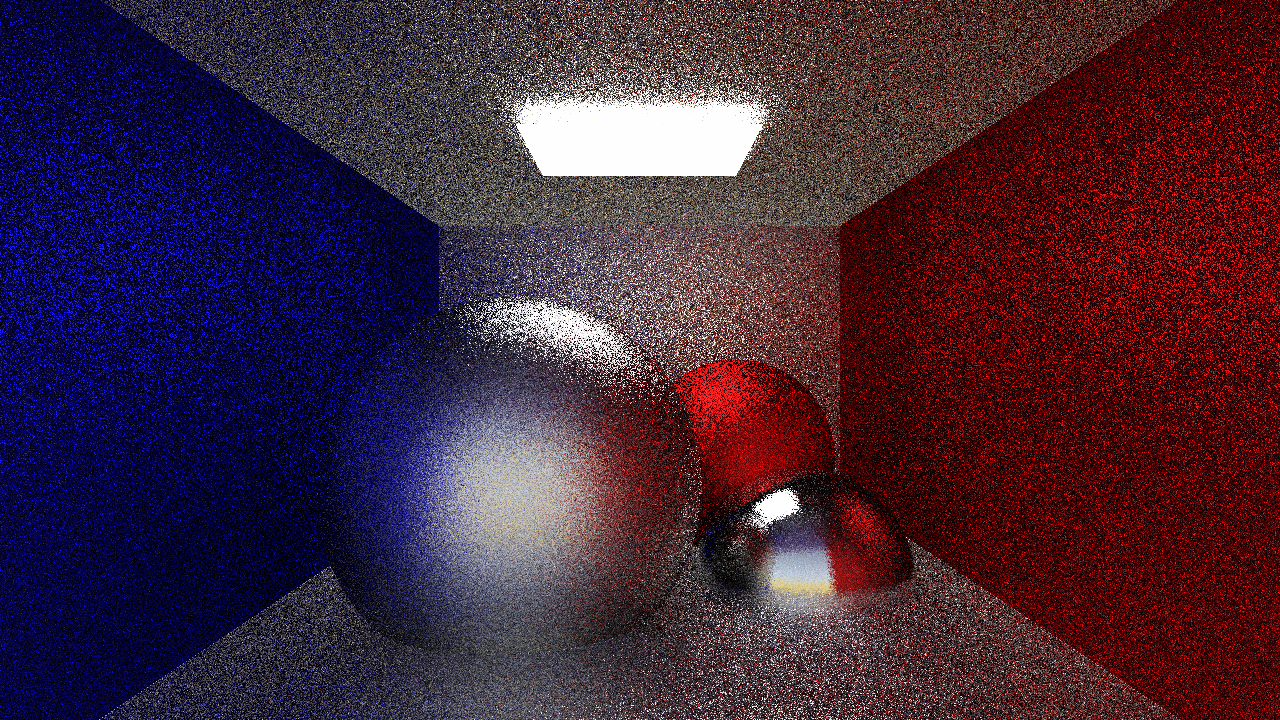
\includegraphics[width=0.7\linewidth]{img/supersampling1.png}
\caption{Supersampling mit einem Schritt}
\label{Supersampling1}
\end{figure}

\begin{figure}[t]
\centering
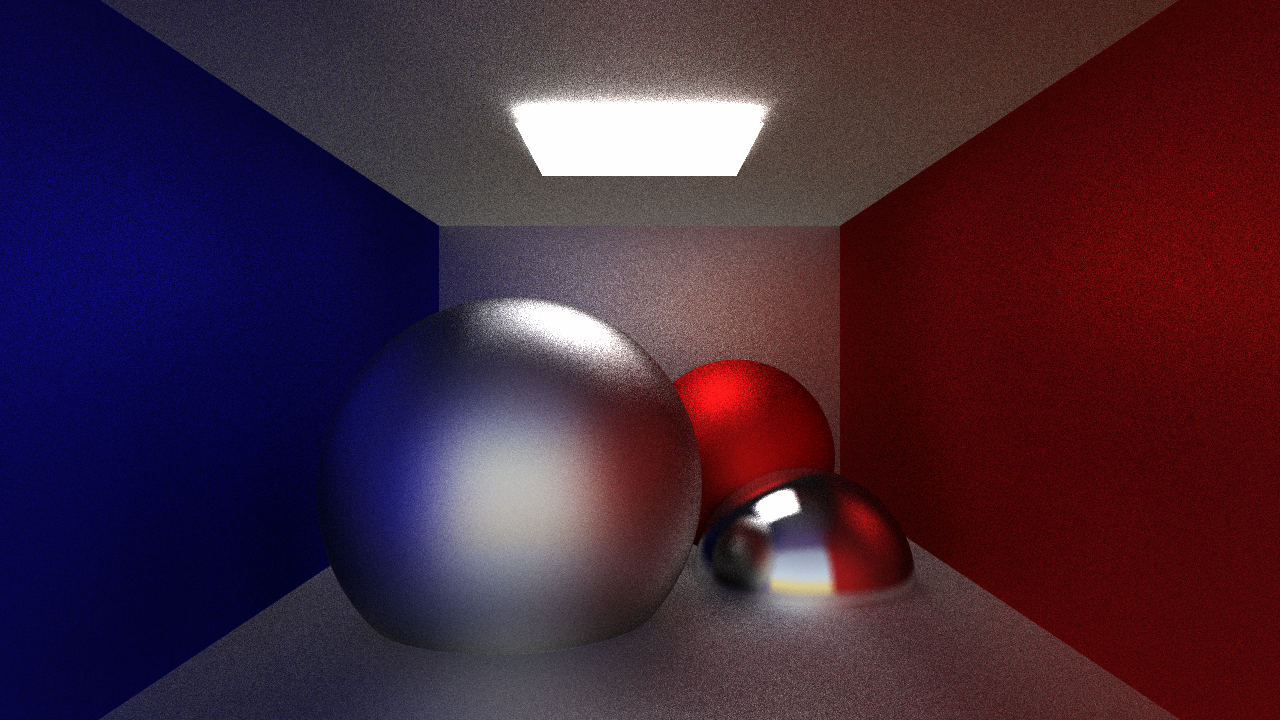
\includegraphics[width=0.7\linewidth]{img/supersampling5.png}
\caption{Supersampling mit fünf Schritten}
\label{Supersampling5}
\end{figure}

Tabelle \ref{Auflösung} zeigt die Auswirkungen verschiedener Auflösungen auf die Laufzeit bei zwei Supersampling-Schritten.
Auch hier wurden wieder drei Messungen für jede Auflösung durchgeführt.

Es lässt sich erkennen, dass die Laufzeit mit steigender Auflösung signifikant ansteigt.
Das Ergebnis ist zu erwarten, denn je höher die Auflösung, desto mehr Pixel müssen berechnet werden, was die Anzahl der Strahlen stark erhöht.
Während die Laufzeit bei 360p noch bei durchschnittlich 0,90 Sekunden liegt, steigt sie bei 1800p auf etwa 22,84 Sekunden an.
\begin{table}[t]
 \caption{Auflösung}

 \label{Auflösung}
 \centering
 \small
 \begin{tabular}[h]{lcccr}
  \toprule
  Resolution & Supersampling Steps & Run1 & Run2 & Run3\\
  \midrule
  360p & 2 & 0.91s & 0.90s & 0.90s\\
  720p & 2 & 3.59s & 3.57s & 3.57s\\
  1080p & 2 & 8.03s & 7.98s & 8.34s\\
  1440p & 2 & 15.19s & 15.24s & 14.43s\\
  1800p & 2 & 23.67s & 22.71s & 22.15s\\
  \bottomrule
 \end{tabular}
\end{table}

In Tabelle \ref{Bounces} wird der Einfluss der maximalen Anzahl an Strahlenreflexionen (Bounces) auf die Laufzeit untersucht.
Hier bleibt die Auflösung konstant bei 720p mit zwei Supersampling-Schritten und 3 Scattern.

Mit zunehmender Anzahl an Reflexionen steigt die Laufzeit deutlich an.
Während die Berechnung bei einem Bounce noch 3,20 Sekunden dauert, erhöht sich die Laufzeit bei fünf Bounces auf durchschnittlich 25,81 Sekunden.
Dies liegt daran, dass bei jeder zusätzlichen Reflexion mehr Berechnungen für die Verfolgung der Strahlen und deren Wechselwirkungen mit den Oberflächen erforderlich sind.
Der Anstieg der Laufzeit ist jedoch nicht linear, da ab einer bestimmten Anzahl an Bounces viele Strahlen absorbiert werden oder keine weiteren Oberflächen mehr treffen, was die zusätzliche Rechenzeit begrenzt.
Abbildung \ref{Bounces1} zeigt das Ergebnis mit einer Reflexion, während Abbildung \ref{Bounces5} das Bild mit fünf Reflexionen darstellt.
Es ist zu erkennen, dass mit zunehmender Anzahl an Bounces mehr indirekte Beleuchtung und Reflexionen sichtbar werden, was zu einer realistischeren Darstellung führt.

\begin{table}[t]
 \caption{Bounces}

 \label{Bounces}
 \centering
 \small
 \begin{tabular}[h]{lcccr}
  \toprule
  Resolution & Bounces & Run1 & Run2 & Run3\\
  \midrule
  720p & 1 & 3.20s & 3.20s & 3.22s\\
  720p & 2 & 3.69s & 3.57s & 3.62s\\
  720p & 3 & 7.54s & 7.46s & 7.43s\\
  720p & 4 & 13.94s & 13.98s & 13.99s\\
  720p & 5 & 25.73s & 25.88s & 25.83s\\
  \bottomrule
 \end{tabular}
\end{table}

Der Parameter Scatter bestimmt die Anzahl der zufällig gestreuten Strahlen an einer Oberfläche.
Die Tabelle \ref{Scatter} veranschaulicht den Einfluss des Scatter-Werts auf die Laufzeit des Raytracers bei einer konstanten Auflösung von 720p.
Der Scatter-Wert bestimmt, wie viele sekundäre Strahlen an einer Oberfläche gestreut werden, um eine realistischere Simulation von diffusen Reflexionen zu erreichen.
Es zeigt sich, dass die Laufzeit mit zunehmendem Scatter-Wert ansteigt.
Während die Berechnung bei einem Scatter im Durchschnitt 3,12 Sekunden benötigt, steigt die Laufzeit bei fünf Scatter-Schritten auf etwa 7,01 Sekunden.
Dies entspricht einem annähernd linearen Anstieg, da mit jedem zusätzlichen Scatter-Wert die Anzahl der verfolgten Strahlen und somit die Rechenzeit zunimmt.
Leichte Abweichungen zwischen den Durchläufen lassen sich durch zufällige Streuungseffekte und die unvorhersehbare Natur der Raytracing-Pfade erklären.

Die Skalierungstests zeigen, dass sowohl eine Erhöhung der Supersampling-Schritte, der Auflösung, der Anzahl der Bounces als auch des Scatter-Werts die Laufzeit signifikant verlängert, wobei der Anstieg oft nicht linear, sondern durch die zunehmende Komplexität der Strahlenverfolgung bedingt ist.
\begin{figure}[t]
\centering
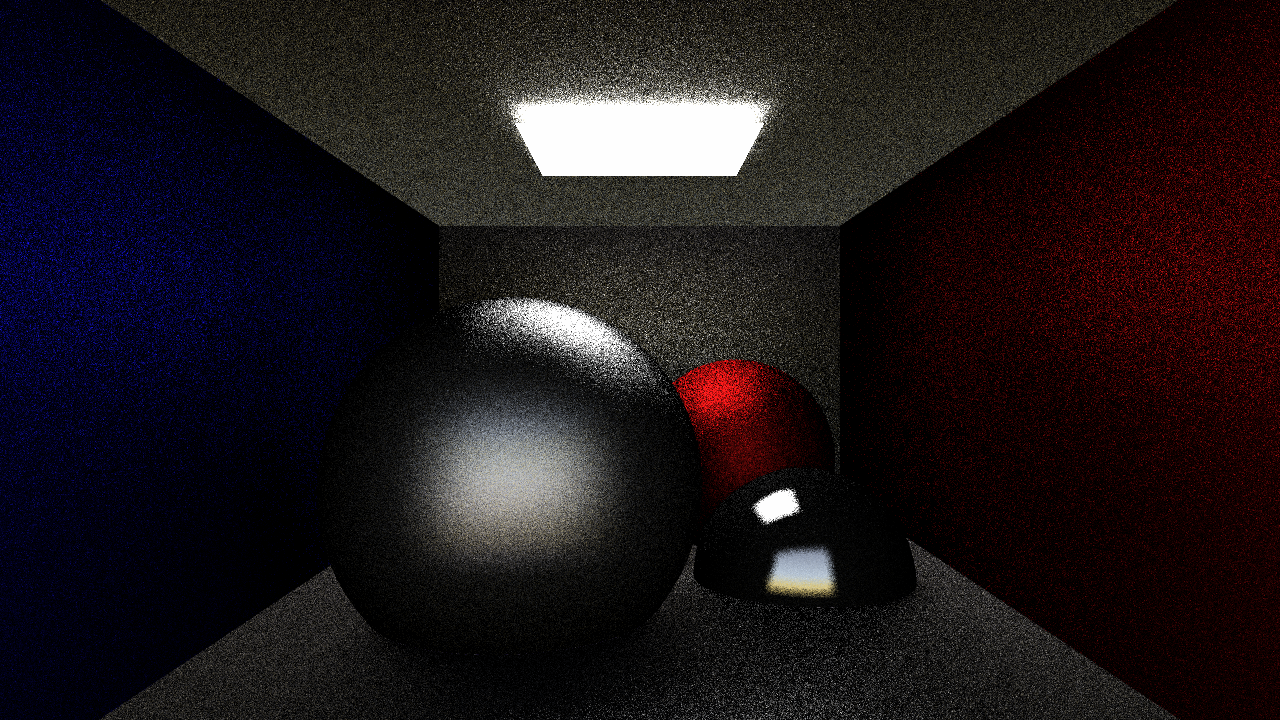
\includegraphics[width=0.7\linewidth]{img/bounce1.png}
\caption{720p mit einer Reflexion}
\label{Bounces1}
\end{figure}

\begin{figure}[t]
\centering
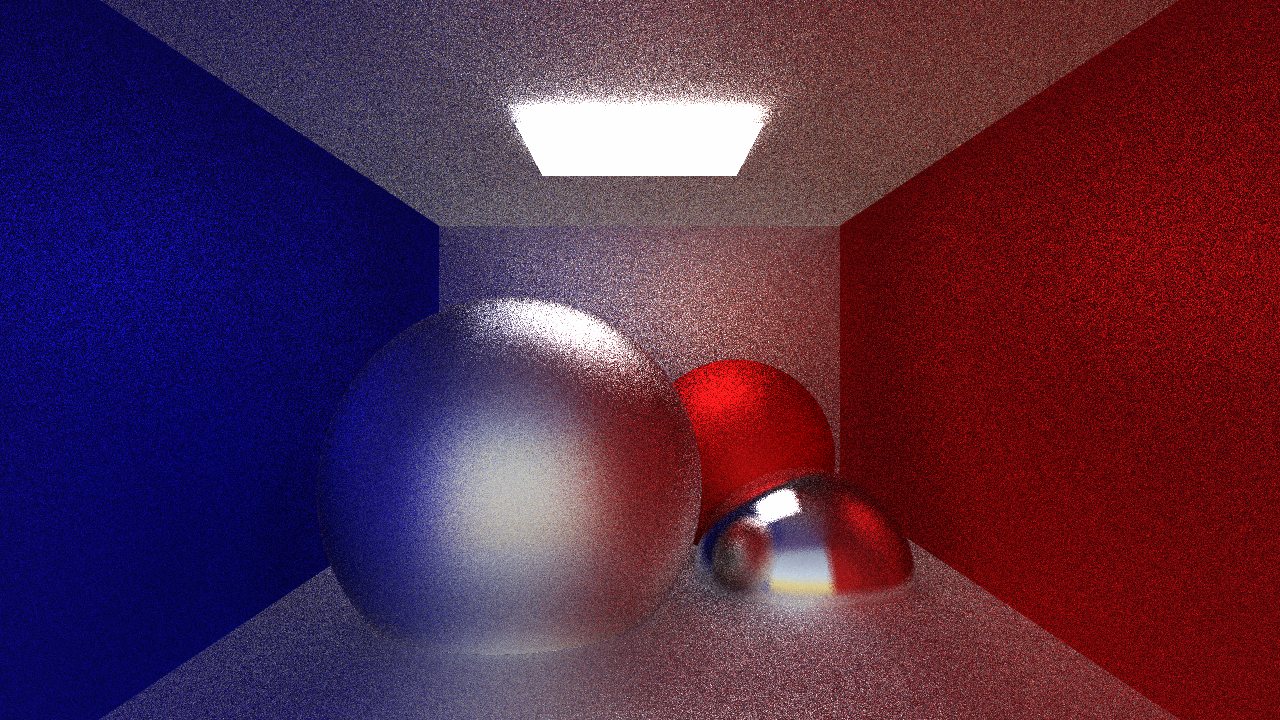
\includegraphics[width=0.7\linewidth]{img/bounce5.png}
\caption{720p mit 5 Reflexionen}
\label{Bounces5}
\end{figure}

\begin{table}[t]
 \caption{Scatter}

 \label{Scatter}
 \centering
 \small
 \begin{tabular}[h]{lcccr}
  \toprule
  Resolution & Scatter & Run1 & Run2 & Run3\\
  \midrule
  720p & 1 & 3.06s & 3.07s & 3.23s\\
  720p & 2 & 2.84s & 2.81s & 2.79s\\
  720p & 3 & 3.77s & 3.57s & 3.56s\\
  720p & 4 & 5.04s & 5.34s & 5.05s\\
  720p & 5 & 7.32s & 6.87s & 6.83s\\
  \bottomrule
 \end{tabular}
\end{table}

\begin{figure}[h]
\centering
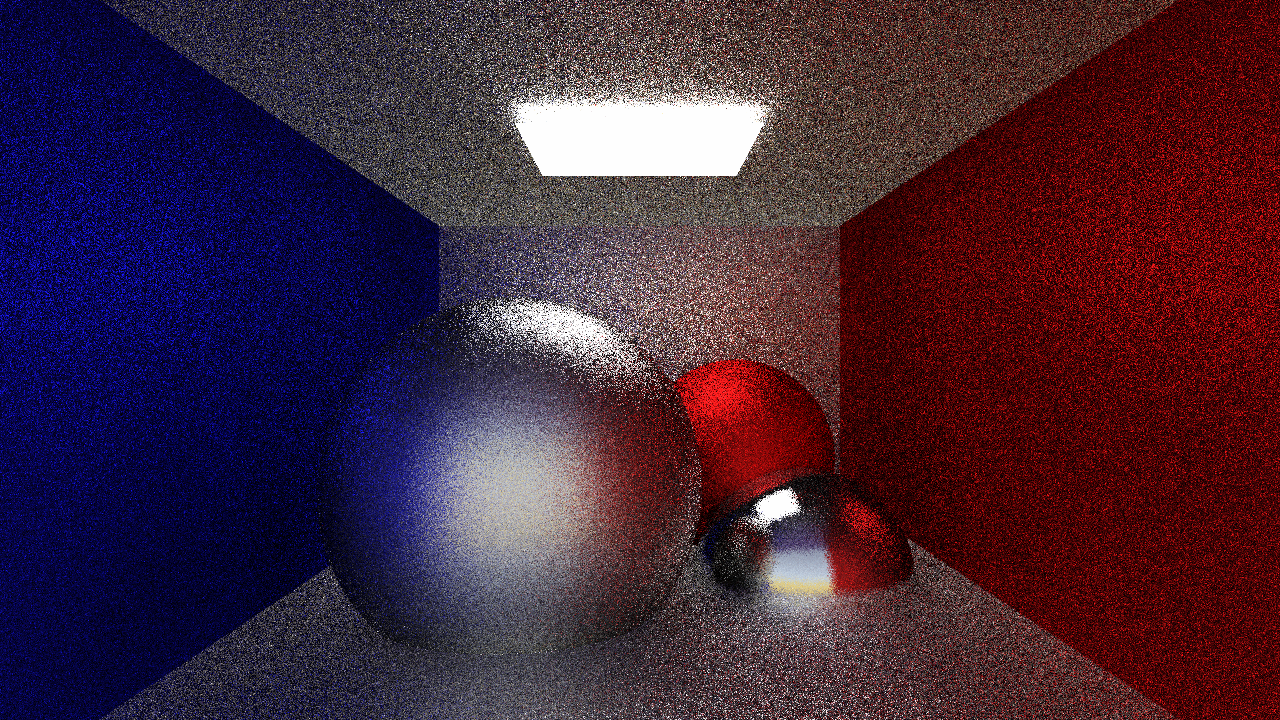
\includegraphics[width=0.7\linewidth]{img/scatter1.png}
\caption{Scatter mit einem Schritt}
\label{Scatter1}
\end{figure}

\begin{figure}[h]
\centering
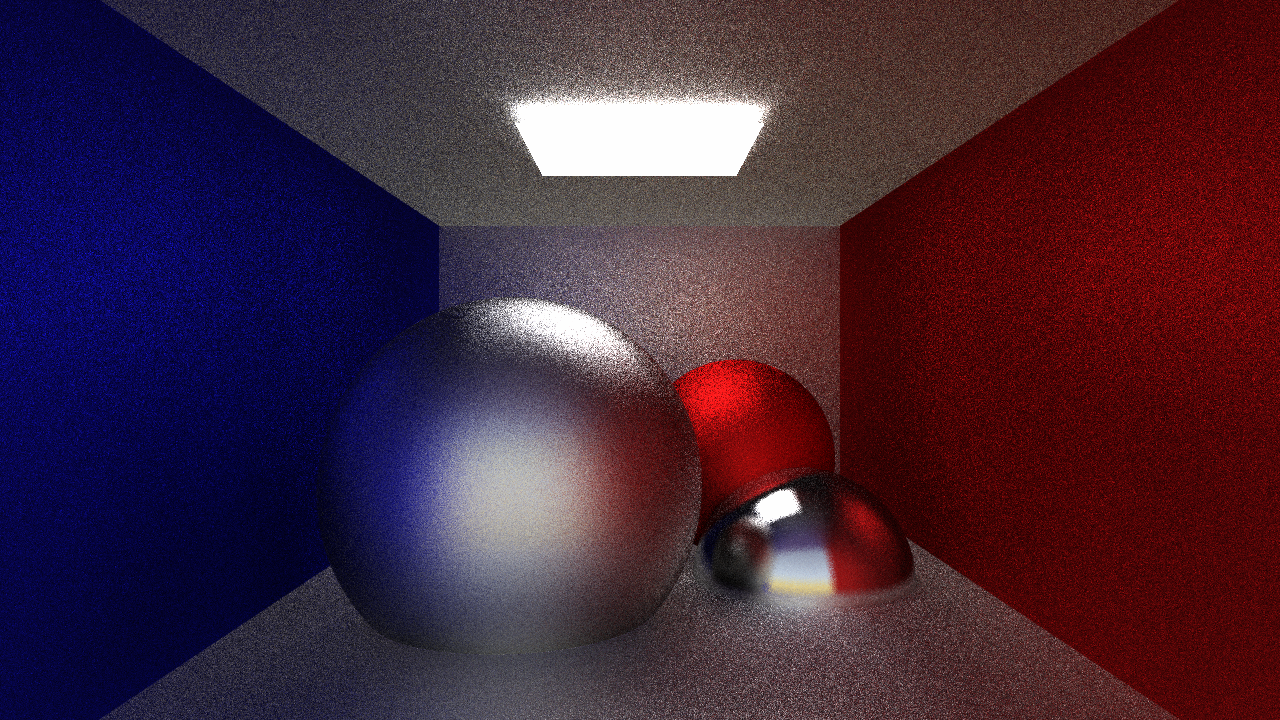
\includegraphics[width=0.7\linewidth]{img/scatter5.png}
\caption{Scatter mit fünf Schritten}
\label{Scatter5}
\end{figure}

\section{Weiterführend}
Der Raytracer ist bereits stark optimiert, allerdings gibt es noch sehr viele weitere Optimierungsverfahren, die allerdings den Rahmen des Projektes übersteigen würden.
Beispielsweise werden die einzelnen Lichtstrahlen noch in einer OOP-Struktur dargestellt und verarbeitet. Durch eine Array-Of-Structures Organisation der Lichtstrahlen könnte man auch hier unnötige Casts und Getter vermeiden und eine effiziente Speichernutzung sicherstellen. Eine Analyse des Programms mittels perf auf Linux zeigt, dass die OOP-Lichtstrahlen im Moment ein Bottleneck darstellen.
Auch das Durchlaufen der gesamten Szene für einen Lichtstrahl ist nicht optimal. Es würde sich ein BVH-Algorithmus anbieten, um nicht alle Objekte der Szene auf Kollisionen checken zu müssen.
Final wäre noch eine GPGPU-Implementierung denkbar, da Raytracer sehr gut parallelisierbar sind. Mit Platformen wie CUDA für Nvidia bzw. ROCm für AMD-Grafikkarten könnte man die Laufzeit des Renderers drastisch reduzieren. 


\section{Fazit} \label{Fazit}
Die vorliegende Arbeit zeigt, dass die Umstellung von einer objektorientierten auf eine datenorientierte Programmierung in Kombination mit Vektorisierung zu einer signifikanten Reduktion der Renderzeit führt.
Die erzielte Optimierung um nahezu 50\% belegt das Potenzial datenorientierter Ansätze in der High-Performance-Computing-Anwendung.
Insbesondere die Nutzung von SIMD-Instruktionen ermöglicht eine effiziente Parallelisierung der Strahlenberechnungen.
Die vollständige Eliminierung der Vec3-Struktur in Kombination mit statischen Methoden hat sich als besonders leistungssteigernd erwiesen.
Ein weiterer Vorteil der datenorientierten Architektur ist die bessere Cache-Nutzung, wodurch sich die Speicherzugriffszeiten minimieren lassen.
Die Ergebnisse verdeutlichen, dass datenorientierte Programmierung in Kombination mit SIMD-Technologie eine vielversprechende Herangehensweise zur Optimierung von Raytracing-Algorithmen darstellt.

Die Skalierungstests zeigen deutlich, dass die Performance des Raytracers stark von der Wahl der Parameter abhängt.
Insbesondere die Erhöhung der Supersampling-Schritte und der Auflösung führt zu einem erheblichen Anstieg der Laufzeit, während die Anzahl der Bounces die Rechenzeit zunehmend beeinflusst.
Der Scatter-Wert wirkt sich sowohl auf die Bildqualität als auch auf die Laufzeit aus, wobei der Anstieg nahezu linear verläuft.
Diese Erkenntnisse bieten wertvolle Ansätze zur Optimierung von Raytracing-Algorithmen, um ein ausgewogenes Verhältnis zwischen Bildqualität und Performance zu erreichen.
\end{document}

